% 74-22(74쪽) — $y=f(x)$ 의 그래프(원문 「오른쪽 그림」). 스캔 화질이 낮아 TikZ 로 다시 그림.
% 라벨은 원문 것만: $2$, $-4$, $\pt{O}$, $\dfrac{\pi}{2}$(화살표), $\pi$, $y=f(x)$. 가로축 단위는 $\pi$ 배.
% 선택지에서 고르는 식은 그림에 적지 않는다.
\begin{tikzpicture}[line width=0.6pt, x=2.20cm, y=0.30cm, >=stealth]
  \draw[densely dashed, line width=0.35pt] (-0.78,2) -- (1.74,2);
  \draw[densely dashed, line width=0.35pt] (-0.78,-4) -- (1.74,-4);
  \draw[densely dashed, line width=0.35pt] (0.5,0) -- (0.5,-4);
  \draw[densely dashed, line width=0.35pt] (1,0) -- (1,2);
  \draw[->, line width=0.7pt] (-0.82,0) -- (1.82,0) node[below=1pt, font=\small] {$x$};
  \draw[->, line width=0.7pt] (0,-6.0) -- (0,3.6) node[left=1pt, font=\small] {$y$};
  \draw[domain=-0.70:1.66, samples=220, smooth] plot (\x, {3*cos(360*\x)-1});
  \node[anchor=east, font=\small, fill=white, inner sep=1pt] at (-0.015,2) {$2$};
  \node[anchor=north east, font=\small, fill=white, inner sep=1pt] at (-0.015,-4) {$-4$};
  \node[anchor=north east, font=\small, fill=white, inner sep=0.5pt] at (-0.01,-0.2) {$\pt{O}$};
  \node[anchor=south, font=\small] at (0.5,2.25) {$\dfrac{\pi}{2}$};
  \draw[->, line width=0.35pt] (0.5,1.80) -- (0.5,0.35);
  \node[anchor=north east, font=\small] at (1.0,-0.2) {$\pi$};
  \node[anchor=south, font=\small] at (1.32,2.25) {$y=f(x)$};
\end{tikzpicture}
